\section*{\hfill \xiaoer\hei{致~~谢} \hfill}
\addcontentsline{toc}{section}{致 谢}
    时光荏苒岁月如梭,转眼自己在HNU的本科生涯就此画上了句号。
    回想过往的憧憬,愈发发觉有涯的人生实在无法穷尽渴望研习讨论的知识,愈发感受到愿景落空后的久萦心间的遗憾。
    \clearpage

% 没有附录的,就不放。
\addcontentsline{toc}{section}{附录}
\addcontentsline{toc}{section}{\song\xiaosi{附录 A}} % 不得不为,如果有就必须要用 \songti 覆盖掉原有的配置 
\section*{附录 A}
    % 需要用 \eqref 才会加圆括号。
    公式推导如 \eqref{eq1} 式所示。
    \begin{equation}
        \begin{aligned}
            \int \frac{x+\sin x}{1 + \cos x} \mathrm{d} x &= \int \frac{x}{2\cos^2 \frac{x}{2}} + \tan \frac{x}{2} \mathrm{d} x \\
                &= \int x\mathrm{d}\tan \frac{x}{2} + \tan \frac{x}{2} \mathrm{d} x \\
                &= \frac{x}{2}\tan \frac{x}{2} - \int \tan \frac{x}{2} \mathrm{d} x + \int \tan \frac{x}{2} \mathrm{d} x \\
                &= x\tan \frac{x}{2} + C 
        \end{aligned}
        \label{eq1}
    \end{equation}
    
    所形成的交换图如图 \ref{fig1},图 \ref{fig2} 和图 \ref{fig3} 所示。
    \begin{figure*}[htp]
        \centering
        \begin{tikzcd}
            A \arrow[r, "\phi"] \arrow[d, red]
            & B \arrow[d, "\psi" red] \\
            C \arrow[r, red, "\eta" blue]
            & |[blue, rotate=-15]| D
        \end{tikzcd}
        % 注意标签一定要放在提供给 ref 的 label 之前否则会出现??.
        \caption{{交换图例一}}
        \label{fig1}
    \end{figure*}
    \begin{figure*}[htp]
        \centering
        \begin{tikzcd}[column sep=tiny]
            & \pi_1(U_1) \ar[dr]\ar[drr, "j_1", bend left=20] &&[1.5em] \\
            \pi_1(U_1\cap U_2) \ar[ur,"i_1"] \ar[dr, "i_2"swap] && \pi_1(U_1) \ast_{\pi_1(U_1\cap U_2)}
            \pi_1(U_2) \ar[r, dashed, "\simeq"] & \pi_1(X) \\
            & \pi_1(U_2) \ar[ur]\ar[urr, "j_2"swap, bend right=20]
            &&
        \end{tikzcd}
        % 手工插入间距
        \vspace{0.5em}\par{\xiaowu{注:关系与图\ref{fig1}类似,但不多.}}
        \caption{{交换图例二}}
        \label{fig2}
    \end{figure*}
    \begin{figure*}[htp]
        \centering
        \begin{tikzcd}
            T
            \arrow[drr, bend left, "x"]
            \arrow[ddr, bend right, "y"]
            \arrow[dr, dotted,background color=blue!20,
            "{(x,y)}"description] & & \\
            & X \times_Z Y \arrow[r, "p"] \arrow[d, "q"]
            & X \arrow[d, "f"] \\
            & Y \arrow[r, "g"]
            & Z
        \end{tikzcd}
        % 手工插入间距
        \vspace{0.5em}\par{\xiaowu{注:关系与图\ref{fig1},图\ref{fig2}类似,但不多.}}
        \caption{{交换图例三}}
        \label{fig3}
    \end{figure*}
    \clearpage
\addcontentsline{toc}{section}{\song\xiaosi{附录 B}}
\section*{附录 B}
    所用图片为图 \ref{fig4}。
    \begin{figure}[htp!]
        \centering
        \begin{subfigure}{0.3\linewidth}
            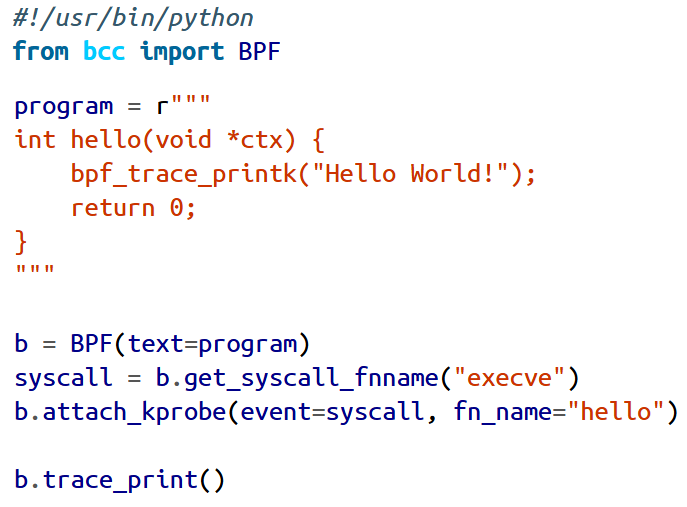
\includegraphics[width=\linewidth]{ebpfProgramExample.png} % 在导言区导入了图片以后,这里就不要再包含后缀名
            \caption{测试代码一}
            \label{f3son1}
        \end{subfigure} 
        \begin{subfigure}{0.3\linewidth}
            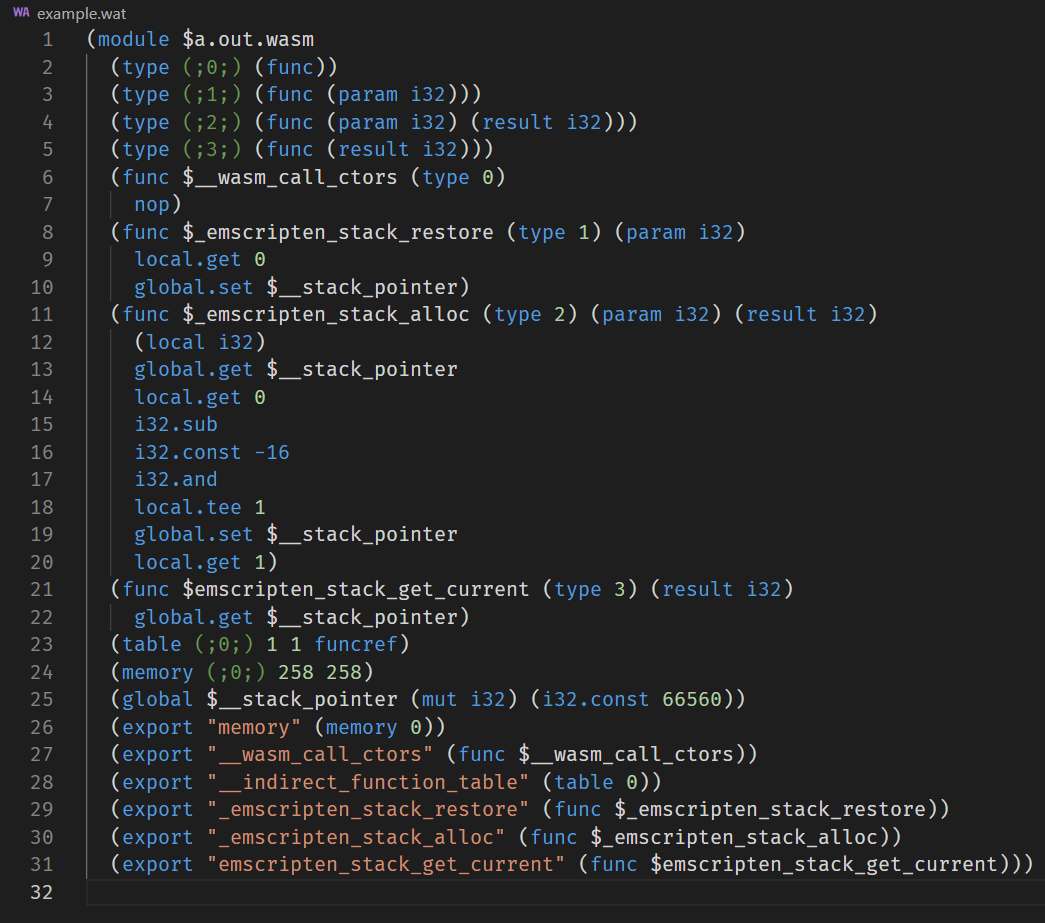
\includegraphics[width=\linewidth]{fig1Codes.png} % 在导言区导入了图片以后,这里就不要再包含后缀名
            \caption{测试代码二}
            \label{f3son2}
        \end{subfigure}
        \caption{所用代码集}
        \label{fig4}
    \end{figure}

    所用表格为表 \ref{tbl1} 和表 \ref{tbl2}。
    \begin{table*}[htp]
        \centering
        \caption{数学字体对照表}
        \begin{threeparttable}
        % resizebox 使表格适应文档的宽度。
        \resizebox{\textwidth}{!}{  
        \xiaowu
        \begin{tabular}{*{18}{l}}
            \toprule
            \multicolumn{2}{c}{\texttt{mathrm}} & \multicolumn{2}{c}{\texttt{mathbf}} & \multicolumn{2}{c}{\texttt{mathit}} & \multicolumn{2}{c}{\texttt{mathsf}} & \multicolumn{2}{c}{\texttt{mathtt}} & \multicolumn{2}{c}{\texttt{mathcal}} & \multicolumn{2}{c}{\texttt{mathbb}} & \multicolumn{2}{c}{\texttt{mathfrak}} & \multicolumn{2}{c}{\texttt{mathscr}} \\ 
            \midrule
            $\mathrm{Aa}$ & $\mathrm{Nn}$ & $\mathbf{Aa}$ & $\mathbf{Nn}$ & $\mathit{Aa}$ & $\mathit{Nn}$ & $\mathsf{Aa}$ & $\mathsf{Nn}$ & $\mathtt{Aa}$ & $\mathtt{Nn}$ & $\mathcal{Aa}$ & $\mathcal{Nn}$ & $\mathbb{A}$ & $\mathbb{N}$ & $\mathfrak{Aa}$ & $\mathfrak{Nn}$ & $\mathscr{Aa}$ & $\mathscr{Nn}$ \\
            $\mathrm{Bb}$ & $\mathrm{Oo}$ & $\mathbf{Bb}$ & $\mathbf{Oo}$ & $\mathit{Bb}$ & $\mathit{Oo}$ & $\mathsf{Bb}$ & $\mathsf{Oo}$ & $\mathtt{Bb}$ & $\mathtt{Oo}$ & $\mathcal{Bb}$ & $\mathcal{Oo}$ & $\mathbb{B}$ & $\mathbb{O}$ & $\mathfrak{Bb}$ & $\mathfrak{Oo}$ & $\mathscr{Bb}$ & $\mathscr{Oo}$ \\
            $\mathrm{Cc}$ & $\mathrm{Pp}$ & $\mathbf{Cc}$ & $\mathbf{Pp}$ & $\mathit{Cc}$ & $\mathit{Pp}$ & $\mathsf{Cc}$ & $\mathsf{Pp}$ & $\mathtt{Cc}$ & $\mathtt{Pp}$ & $\mathcal{Cc}$ & $\mathcal{Pp}$ & $\mathbb{C}$ & $\mathbb{P}$ & $\mathfrak{Cc}$ & $\mathfrak{Pp}$ & $\mathscr{Cc}$ & $\mathscr{Pp}$ \\
            $\mathrm{Dd}$ & $\mathrm{Qq}$ & $\mathbf{Dd}$ & $\mathbf{Qq}$ & $\mathit{Dd}$ & $\mathit{Qq}$ & $\mathsf{Dd}$ & $\mathsf{Qq}$ & $\mathtt{Dd}$ & $\mathtt{Qq}$ & $\mathcal{Dd}$ & $\mathcal{Qq}$ & $\mathbb{D}$ & $\mathbb{Q}$ & $\mathfrak{Dd}$ & $\mathfrak{Qq}$ & $\mathscr{Dd}$ & $\mathscr{Qq}$ \\
            $\mathrm{Ee}$ & $\mathrm{Rr}$ & $\mathbf{Ee}$ & $\mathbf{Rr}$ & $\mathit{Ee}$ & $\mathit{Rr}$ & $\mathsf{Ee}$ & $\mathsf{Rr}$ & $\mathtt{Ee}$ & $\mathtt{Rr}$ & $\mathcal{Ee}$ & $\mathcal{Rr}$ & $\mathbb{E}$ & $\mathbb{R}$ & $\mathfrak{Ee}$ & $\mathfrak{Rr}$ & $\mathscr{Ee}$ & $\mathscr{Rr}$ \\
            $\mathrm{Ff}$ & $\mathrm{Ss}$ & $\mathbf{Ff}$ & $\mathbf{Ss}$ & $\mathit{Ff}$ & $\mathit{Ss}$ & $\mathsf{Ff}$ & $\mathsf{Ss}$ & $\mathtt{Ff}$ & $\mathtt{Ss}$ & $\mathcal{Ff}$ & $\mathcal{Ss}$ & $\mathbb{F}$ & $\mathbb{S}$ & $\mathfrak{Ff}$ & $\mathfrak{Ss}$ & $\mathscr{Ff}$ & $\mathscr{Ss}$ \\
            $\mathrm{Gg}$ & $\mathrm{Tt}$ & $\mathbf{Gg}$ & $\mathbf{Tt}$ & $\mathit{Gg}$ & $\mathit{Tt}$ & $\mathsf{Gg}$ & $\mathsf{Tt}$ & $\mathtt{Gg}$ & $\mathtt{Tt}$ & $\mathcal{Gg}$ & $\mathcal{Tt}$ & $\mathbb{G}$ & $\mathbb{T}$ & $\mathfrak{Gg}$ & $\mathfrak{Tt}$ & $\mathscr{Gg}$ & $\mathscr{Tt}$ \\
            $\mathrm{Hh}$ & $\mathrm{Uu}$ & $\mathbf{Hh}$ & $\mathbf{Uu}$ & $\mathit{Hh}$ & $\mathit{Uu}$ & $\mathsf{Hh}$ & $\mathsf{Uu}$ & $\mathtt{Hh}$ & $\mathtt{Uu}$ & $\mathcal{Hh}$ & $\mathcal{Uu}$ & $\mathbb{H}$ & $\mathbb{U}$ & $\mathfrak{Hh}$ & $\mathfrak{Uu}$ & $\mathscr{Hh}$ & $\mathscr{Uu}$ \\
            $\mathrm{Ii}$ & $\mathrm{Vv}$ & $\mathbf{Ii}$ & $\mathbf{Vv}$ & $\mathit{Ii}$ & $\mathit{Vv}$ & $\mathsf{Ii}$ & $\mathsf{Vv}$ & $\mathtt{Ii}$ & $\mathtt{Vv}$ & $\mathcal{Ii}$ & $\mathcal{Vv}$ & $\mathbb{I}$ & $\mathbb{V}$ & $\mathfrak{Ii}$ & $\mathfrak{Vv}$ & $\mathscr{Ii}$ & $\mathscr{Vv}$ \\
            $\mathrm{Jj}$ & $\mathrm{Ww}$ & $\mathbf{Jj}$ & $\mathbf{Ww}$ & $\mathit{Jj}$ & $\mathit{Ww}$ & $\mathsf{Jj}$ & $\mathsf{Ww}$ & $\mathtt{Jj}$ & $\mathtt{Ww}$ & $\mathcal{Jj}$ & $\mathcal{Ww}$ & $\mathbb{J}$ & $\mathbb{W}$ & $\mathfrak{Jj}$ & $\mathfrak{Ww}$ & $\mathscr{Jj}$ & $\mathscr{Ww}$ \\
            $\mathrm{Kk}$ & $\mathrm{Xx}$ & $\mathbf{Kk}$ & $\mathbf{Xx}$ & $\mathit{Kk}$ & $\mathit{Xx}$ & $\mathsf{Kk}$ & $\mathsf{Xx}$ & $\mathtt{Kk}$ & $\mathtt{Xx}$ & $\mathcal{Kk}$ & $\mathcal{Xx}$ & $\mathbb{K}$ & $\mathbb{X}$ & $\mathfrak{Kk}$ & $\mathfrak{Xx}$ & $\mathscr{Kk}$ & $\mathscr{Xx}$ \\
            $\mathrm{Ll}$ & $\mathrm{Yy}$ & $\mathbf{Ll}$ & $\mathbf{Yy}$ & $\mathit{Ll}$ & $\mathit{Yy}$ & $\mathsf{Ll}$ & $\mathsf{Yy}$ & $\mathtt{Ll}$ & $\mathtt{Yy}$ & $\mathcal{Ll}$ & $\mathcal{Yy}$ & $\mathbb{L}$ & $\mathbb{Y}$ & $\mathfrak{Ll}$ & $\mathfrak{Yy}$ & $\mathscr{Ll}$ & $\mathscr{Yy}$ \\
            $\mathrm{Mm}$ & $\mathrm{Zz}$ & $\mathbf{Mm}$ & $\mathbf{Zz}$ & $\mathit{Mm}$ & $\mathit{Zz}$ & $\mathsf{Mm}$ & $\mathsf{Zz}$ & $\mathtt{Mm}$ & $\mathtt{Zz}$ & $\mathcal{Mm}$ & $\mathcal{Zz}$ & $\mathbb{M}$ & $\mathbb{Z}$ & $\mathfrak{Mm}$ & $\mathfrak{Zz}$ & $\mathscr{Mm}$ & $\mathscr{Zz}$ \\
            \bottomrule
        \end{tabular}
        }
        \begin{tablenotes}
            \item \xiaowu\songti{注:此数据仅为示例,实际数据可能有所不同.}
        \end{tablenotes}
        \end{threeparttable}
        \label{tbl1}
    \end{table*}
    \begin{table}[H]
        \centering
        \caption{各组分 $\lg(B_i)$ 值}
        \wuhao
        \begin{tabular}{ccccc} 
            \hline
            % 视需求套上斜体。
            序号 & \multicolumn{2}{c}{T=1500K} & \multicolumn{2}{c}{T=2000K}  \\ 
            \cline{2-5}
            & 组分                   & $\lg B_i$   & 组分                  & $\lg B_i$ \\ 
            \hline
            1  & \ce{O2}\TblrNote{+}   &   5.26      & \ce{HO2}              &  6.43    \\
            2  & \ce{HO2}              &   5.26      & \ce{O2}\TblrNote{+}   &  6.42    \\
            3  & \ce{H2O}\TblrNote{+}  &   4.76      & \ce{H2O}\TblrNote{+}  &  6.18    \\
            4  & \ce{N2}\TblrNote{+}   &   3.97      & \ce{H}                &  6.12    \\
            5  & \ce{H}                &   3.54      & \ce{H2}\TblrNote{+}   &  6.04    \\
            6  & \ce{OH}               &   3.29      & \ce{OH}               &  5.91    \\
            7  & \ce{CO}\TblrNote{+}   &   3.26      & \ce{O}                &  5.59    \\
            8  & \ce{H2}\TblrNote{+}   &   2.54      & \ce{N2}\TblrNote{+}   &  4.87    \\
            9  & \ce{O}                &   2.30      & \ce{CO}\TblrNote{+}   &  3.98    \\
            10 & \ce{H2O2}             &   1.62      & \ce{CO2}\TblrNote{+}  &  3.76    \\
            11 & \ce{CO2}\TblrNote{+}  &   1.40      & \ce{H2O2}             &  3.09    \\
            12 & \ce{HCO}\TblrNote{*}  &   -0.47     & \ce{HCO}\TblrNote{*}  &  0.24    \\
            13 & \ce{N}\TblrNote{+}    &   -4.85     & \ce{N}\TblrNote{+}    &  -2.81   \\
            14 & \ce{CH2O}\TblrNote{+} &   -6.91     & \ce{CH2O}\TblrNote{*} &  -6.13   \\
            15 & \ce{NO}\TblrNote{+}   &   -16.60    & \ce{NO}\TblrNote{+}   &  -11.76  \\ 
            \hline
            \multicolumn{5}{l}{\xiaowu\songti{注:“+”表示重要成分,“*”表示冗余组分.}}                      
        \end{tabular}
        \label{tbl2}
    \end{table}